% !TeX program = xelatex
% UTF-8. Compile twice with XeLaTeX.
\documentclass[UTF8,a4paper,zihao=5,fontset=none]{ctexart}
\usepackage[left=23mm,right=23mm,top=20mm,bottom=21mm,footskip=10mm]{geometry}
\usepackage{fontspec}
\setmainfont{Times New Roman}
\setsansfont{Times New Roman}
\setmonofont{Consolas}[Scale=0.91]
\newfontfamily{\circledfont}{Segoe UI Symbol}
\setCJKmainfont{SimSun}[AutoFakeBold=2]
\setCJKsansfont{SimHei}
\setCJKmonofont{SimSun}
\setCJKfamilyfont{hei}{SimHei}
\newcommand{\heiti}{\CJKfamily{hei}}
\usepackage{amsmath,amssymb,array,booktabs,longtable,tabularx,makecell}
\usepackage{graphicx,tikz,caption,listings,needspace}
\usetikzlibrary{arrows.meta,positioning,calc}
\usepackage[hidelinks,unicode,pdfencoding=auto]{hyperref}
\hypersetup{pdftitle={作业3 GPIO工作原理与寄存器编程},pdfauthor={彭俊杰},pdfsubject={嵌入式系统课程作业}}
\ctexset{
  section={format=\heiti\fontsize{11.5}{16.5}\selectfont,number=\arabic{section}.,aftername=\hspace{0.4em},beforeskip=11pt,afterskip=8pt},
  subsection={format=\heiti\fontsize{11}{16}\selectfont,number={{\circledfont\ifcase\value{subsection}\or①\or②\or③\or④\fi}},aftername=\hspace{0.4em},beforeskip=10pt,afterskip=7pt}
}
\pdfstringdefDisableCommands{\def\circledfont{}}
\linespread{1.22}
\setlength{\parindent}{2em}
\setlength{\parskip}{3pt}
\setlength{\emergencystretch}{1.5em}
\raggedbottom
\pagestyle{plain}
\clubpenalty=10000
\widowpenalty=10000
\displaywidowpenalty=10000
\captionsetup{font=small,labelsep=quad,justification=centering,singlelinecheck=false,hypcap=false,skip=6pt}
\newcolumntype{L}[1]{>{\raggedright\arraybackslash}m{#1}}
\newcolumntype{C}[1]{>{\centering\arraybackslash}m{#1}}
\newcolumntype{Y}{>{\raggedright\arraybackslash}X}
\newcolumntype{Z}{>{\centering\arraybackslash}X}
\renewcommand{\tabularxcolumn}[1]{m{#1}}
\newcommand{\TableHead}[1]{\multicolumn{1}{c}{\heiti #1}}
\newcommand{\hex}[1]{\texttt{0x#1}}
\newcommand{\code}[1]{\texttt{#1}}
\newcommand{\question}[1]{\begingroup\linespread{1}\fontsize{10.5}{15.5}\selectfont\noindent\textbf{题目}\quad #1\par\endgroup\vspace{4pt}}
\newenvironment{datatab}{\par\begingroup\centering\linespread{1}\fontsize{10.5}{14.5}\selectfont\setlength{\tabcolsep}{5pt}\renewcommand{\arraystretch}{1.14}\setlength{\extrarowheight}{2pt}}{\par\endgroup\vspace{5pt}}
\tikzset{
  block/.style={draw=black!70,fill=black!3,line width=0.55pt,align=center,inner sep=5pt,font=\linespread{1}\fontsize{10.5}{14.5}\selectfont},
  arrow/.style={-{Stealth[length=2mm]},line width=0.7pt},
  wire/.style={line width=0.65pt}
}
\lstdefinestyle{cstyle}{
  language=C,basicstyle=\linespread{1}\ttfamily\fontsize{9.4}{11.7}\selectfont,
  keywordstyle=\bfseries,commentstyle=\normalfont,
  stringstyle=\ttfamily,numbers=left,numberstyle=\ttfamily\fontsize{7.5}{10}\selectfont,
  numbersep=8pt,xleftmargin=19pt,xrightmargin=1pt,
  showstringspaces=false,tabsize=4,keepspaces=true,columns=fullflexible,
  breaklines=true,breakatwhitespace=true,aboveskip=5pt,belowskip=7pt,
  frame=none,captionpos=t
}
\lstset{style=cstyle}
% —— 第2题流向标注配色 ——
\definecolor{inblue}{RGB}{0,90,200}
\definecolor{outred}{RGB}{205,0,0}
\definecolor{cfggray}{RGB}{90,90,90}

\begin{document}
\begin{center}
  {\heiti\fontsize{22}{28}\selectfont 作业3\par}
  \vspace{3pt}
  {\heiti\fontsize{13}{18}\selectfont GPIO工作原理与寄存器编程\par}
  \vspace{5pt}
  {\fontsize{11}{16}\selectfont 彭俊杰\qquad 智装备241\qquad 2024306100324\par}
\end{center}
\vspace{-3pt}

\section{请解释\code{GPIOD\_BASE}的地址计算方法，并说明\code{GPIOD->OTYPER}寄存器的地址是多少？}

\subsection{\code{GPIOD\_BASE} 的计算}

STM32F40x 的 GPIO 挂在 AHB1 总线上。求 GPIOD 的基址时，先从片上外设区首地址 \hex{4000\,0000} 加上 AHB1 外设区的偏移 \hex{0002\,0000}，得到 \hex{4002\,0000}，再加上 GPIOD 在该区内的偏移。

GPIOA、GPIOB、GPIOC、GPIOD 的基址依次相隔 \hex{0400}，也就是 1 KB。若从 GPIOA 开始按 0、1、2、3 编号，GPIOD 的偏移就是 $3\times\hex{0400}=\hex{0C00}$。计算如下：

\begin{datatab}
\begin{tabular}{@{}C{48mm}L{80mm}C{24mm}@{}}
\toprule
\TableHead{层级} & \TableHead{计算式} & \TableHead{结果}\\
\midrule
片上外设区首地址 & \code{PERIPH\_BASE} & \hex{4000\,0000}\\
AHB1 外设区首地址 & \hex{4000\,0000} $+$ \hex{0002\,0000} & \hex{4002\,0000}\\
GPIOD 基址 & \hex{4002\,0000} $+$ $3\times\hex{0400}$ & \textbf{\hex{4002\,0C00}}\\
\bottomrule
\end{tabular}
\end{datatab}

对应的地址宏为：

\begin{lstlisting}[language=C]
#define PERIPH_BASE        0x40000000UL
#define AHB1PERIPH_BASE    (PERIPH_BASE + 0x00020000UL)
#define GPIOD_BASE         (AHB1PERIPH_BASE + 0x0C00UL)
\end{lstlisting}

\begin{datatab}
\begin{tabular}{@{}C{12mm}L{31mm}C{12mm}L{31mm}C{12mm}L{31mm}@{}}
\toprule
\TableHead{端口} & \TableHead{基址} & \TableHead{端口} & \TableHead{基址} & \TableHead{端口} & \TableHead{基址}\\
\midrule
GPIOA & \hex{4002\,0000} & GPIOD & \textbf{\hex{4002\,0C00}} & GPIOG & \hex{4002\,1800}\\
GPIOB & \hex{4002\,0400} & GPIOE & \hex{4002\,1000} & GPIOH & \hex{4002\,1C00}\\
GPIOC & \hex{4002\,0800} & GPIOF & \hex{4002\,1400} & GPIOI & \hex{4002\,2000}\\
\bottomrule
\end{tabular}
\end{datatab}

GPIOD 的地址区间为 \hex{4002\,0C00} $\sim$ \hex{4002\,0FFF}，共 1 KB，包括寄存器地址和保留地址。

\subsection{\code{GPIOD->OTYPER} 的地址}

\code{OTYPER} 是输出类型寄存器，在端口内的偏移为 \hex{04}。所以它的地址为
\[
  \hex{4002\,0C00}+\hex{04}=\boxed{\hex{4002\,0C04}}\,.
\]

头文件用 \code{GPIO\_TypeDef} 描述寄存器的排列，\code{GPIOD} 则是指向它的指针。以下列出结构体的前两个成员和指针定义：

\begin{lstlisting}[language=C]
__IO uint32_t MODER;    /* 偏移 0x00 */
__IO uint32_t OTYPER;   /* 偏移 0x04 */
#define GPIOD  ((GPIO_TypeDef *) GPIOD_BASE)
\end{lstlisting}

\code{MODER} 占 4 字节，所以紧随其后的 \code{OTYPER} 位于基址加 4 字节处。\textbf{\code{\&GPIOD->OTYPER} 的地址值为 \hex{4002\,0C04}}，\code{GPIOD->OTYPER} 访问该地址处的寄存器内容。

\newpage

\section{STM32F40x 系列芯片的 GPIO 端口若作为通用数字输入或输出模式，则分别需要设置哪些寄存器？请在位结构工作原理图上画出两者的流向和所用寄存器。}

\subsection{寄存器设置}

配置前，先在 \code{RCC\_AHB1ENR} 中使能相应 GPIO 端口的时钟。例如使用 GPIOD 时，将第 3 位 \code{GPIODEN} 置 1。

\textbf{通用数字输入}设置 \code{MODER} 和 \code{PUPDR}，从 \code{IDR} 读取引脚状态；\textbf{通用数字输出}设置 \code{MODER}、\code{OTYPER}、\code{OSPEEDR}，按电路需要选择 \code{PUPDR}，再写 \code{ODR} 或 \code{BSRR} 控制输出电平。各寄存器的作用见下表：

\begin{datatab}
\begin{tabular}{@{}L{38mm}L{50mm}L{64mm}@{}}
\toprule
\TableHead{寄存器} & \TableHead{通用数字输入} & \TableHead{通用数字输出}\\
\midrule
\code{GPIOx\_MODER}\newline 模式 & 对应引脚的两位设为 \code{00} & 对应引脚的两位设为 \code{01}\\
\code{GPIOx\_OTYPER}\newline 输出类型 & 输出驱动器关闭，无须配置 & 对应引脚的一位：\code{0} 推挽，\code{1} 开漏\\
\code{GPIOx\_OSPEEDR}\newline 输出速度 & 不影响输入通路，无须配置 & 对应两位：\code{00} 低速，\code{01} 中速，\code{10} 高速，\code{11} 超高速\\
\code{GPIOx\_PUPDR}\newline 上拉/下拉 & 对应两位：\code{00} 无上/下拉（浮空），\code{01} 上拉，\code{10} 下拉 & 按电路需要选无上/下拉、上拉或下拉；编码与输入模式相同\\
\code{GPIOx\_IDR}\newline 输入数据 & 读取对应位，得到引脚电平 & 也可读取，用于查看实际引脚电平\\
\code{GPIOx\_ODR}\newline 输出数据 & 不用于控制输入电平 & 写对应位：\code{0} 或 \code{1}，保存待输出的数据\\
\code{GPIOx\_BSRR}\newline 位设置/复位 & 不用于控制输入电平 & 按位置位或复位 \code{ODR}，可代替直接修改 \code{ODR}\\
\bottomrule
\end{tabular}
\end{datatab}

表中的设置值针对单个引脚。对引脚 $y$（$y=0\sim15$），\code{MODER}、\code{OSPEEDR}、\code{PUPDR} 都使用第 $2y+1:2y$ 位，\code{OTYPER}、\code{IDR}、\code{ODR} 使用第 $y$ 位。例如配置 PD3 时，将 \code{GPIOD->MODER} 的第 7:6 位设为 \code{00} 即为输入，设为 \code{01} 即为通用输出。

\subsection{输入和输出的工作过程}

\textbf{输入模式：}输出驱动器关闭，施密特触发器开启。外部信号从 I/O 引脚进入，经过施密特触发器形成数字电平，每个 AHB1 时钟周期采样到 \code{IDR}。程序读 \code{IDR} 的对应位，就得到引脚状态。\code{PUPDR} 控制弱上拉或弱下拉；当外部电路没有驱动引脚时，它们可使输入保持确定的电平。

\textbf{输出模式：}程序直接写 \code{ODR}，或写 \code{BSRR} 修改 \code{ODR} 的相应位。该值经过通用输出通路和输出控制电路，控制 P-MOS、N-MOS，最后作用于引脚。\code{MODER} 选择通用输出通路，\code{OTYPER} 决定推挽或开漏，\code{OSPEEDR} 选择输出速度等级，影响信号边沿的上升和下降速度。

\textbf{推挽与开漏：}推挽输出时，\code{ODR} 为 1 时 P-MOS 导通、N-MOS 关闭，输出高电平；为 0 时 N-MOS 导通、P-MOS 关闭，输出低电平。开漏输出时，P-MOS 始终关闭；\code{ODR} 为 0 时 N-MOS 导通，拉低引脚，为 1 时 N-MOS 也关闭，引脚呈高阻态。此时要得到高电平，需要上拉电阻，可按负载和速度要求采用内部弱上拉或外部上拉。

\newpage
\subsection{位结构图中的流向}

图~\ref{fig:bitstruct} 中，蓝色箭头表示输入信号的流向，红色箭头表示输出数据的流向，灰色虚线指向配置寄存器控制的电路。

\begin{figure}[htbp]
\centering
\begin{tikzpicture}
  \node[anchor=south west,inner sep=0] (fig) at (0,0)
    {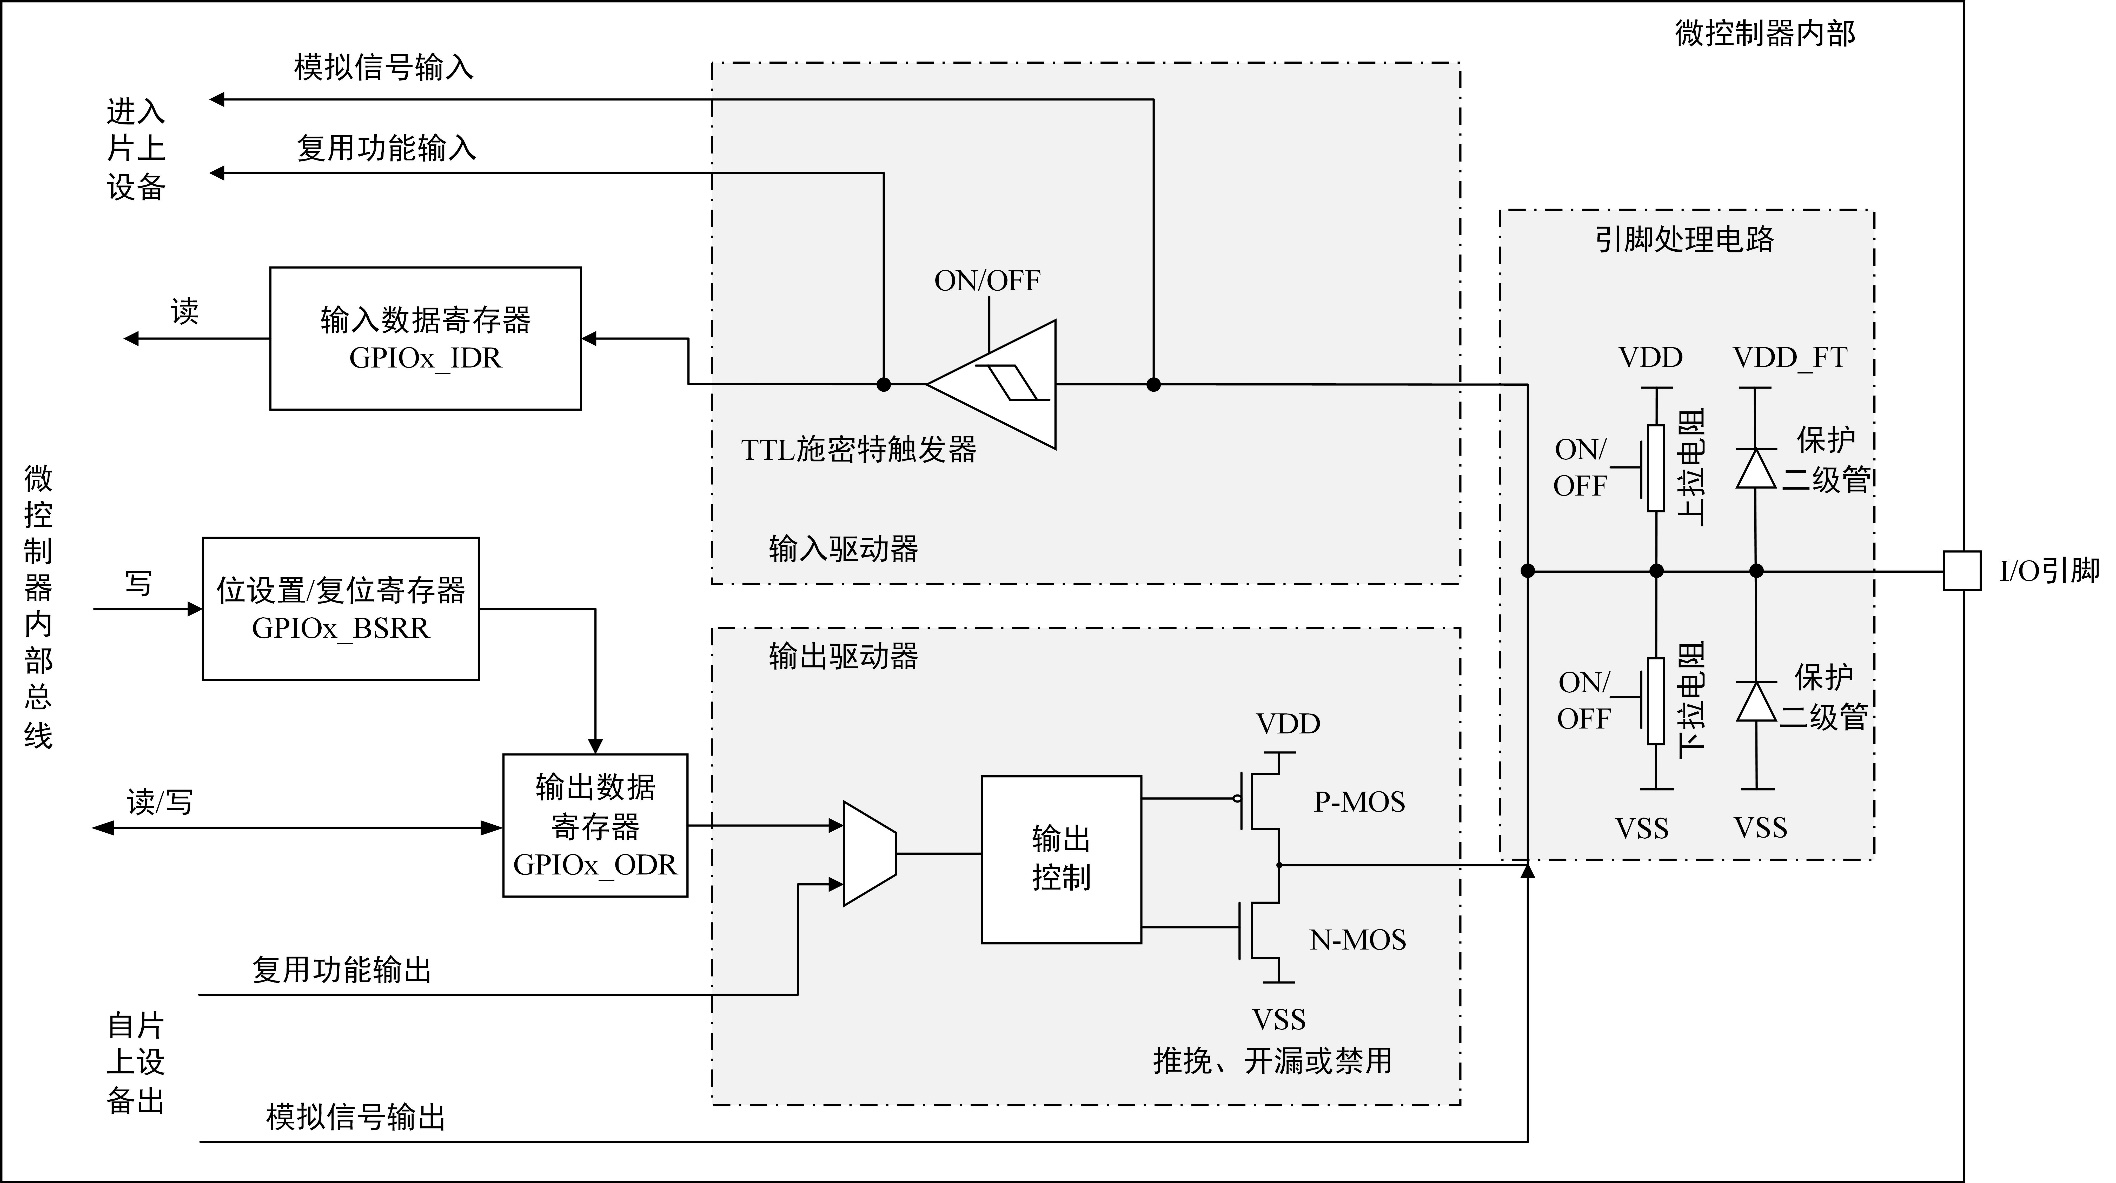
\includegraphics[width=164mm]{latex_assets/figure5-1_GPIO-bit-structure_lecture05-1-slide.jpg}};
  \begin{scope}[shift={(fig.south west)},x=0.0775mm,y=0.0775mm,
      flowin/.style={preaction={draw=white,line width=2.4pt},draw=inblue,line width=1.3pt,line cap=round,line join=round},
      flowout/.style={preaction={draw=white,line width=2.4pt},draw=outred,line width=1.3pt,line cap=round,line join=round},
      cfgpoint/.style={-{Stealth[length=1.9mm]},draw=cfggray,line width=0.55pt,dashed},
      lblbox/.style={fill=white,fill opacity=0.92,draw=black!35,line width=0.4pt,rounded corners=1.5pt,
                     inner sep=2.5pt,align=center,text opacity=1,
                     font=\linespread{1.05}\ttfamily\fontsize{8}{10.2}\selectfont}]
    % —— 输入流向（蓝 1）：引脚 → 施密特触发器 → IDR → 总线读 ——
    \draw[flowin,-{Stealth[length=2.6mm]}] (1940,625) -- (1528,625) -- (1528,799) -- (1065,799);
    \draw[flowin,-{Stealth[length=2.6mm]}] (924,799) -- (685,799) -- (685,848) -- (592,848);
    \draw[flowin,-{Stealth[length=2.6mm]}] (262,848) -- (134,848);   % IDR → 总线“读”
    % —— 输出流向（红 2）：总线写 → BSRR/ODR → 输出控制 → P/N-MOS → 引脚 ——
    \draw[flowout,-{Stealth[length=2.6mm]}] (132,575) -- (198,575);  % 写 → BSRR
    \draw[flowout,-{Stealth[length=2.6mm]}] (486,575) -- (592,575) -- (592,441); % BSRR → ODR
    \draw[flowout,-{Stealth[length=2.6mm]}] (130,358) -- (500,358);  % 读/写 → ODR
    \draw[flowout,-{Stealth[length=2.1mm]}] (694,358) -- (840,358); % ODR → 通路选择
    \draw[flowout,-{Stealth[length=2.1mm]}] (898,332) -- (982,332); % 通路选择 → 输出控制
    \draw[flowout,-{Stealth[length=2.1mm]}] (1155,384) -- (1248,384); % P-MOS 控制
    \draw[flowout,-{Stealth[length=2.1mm]}] (1155,254) -- (1248,254); % N-MOS 控制
    \draw[flowout,-{Stealth[length=2.6mm]}] (1282,318) -- (1528,318)
         -- (1528,601) -- (1940,601);                % MOS 公共节点 → 引脚
    % —— 配置寄存器指示（灰）——
    \draw[cfgpoint] (660,702) -- (780,900) -- (1004,860); % MODER → 输入使能
    \draw[cfgpoint] (660,634) -- (724,600) -- (724,467) -- (868,467) -- (868,388); % 通路选择
    \draw[cfgpoint] (1448,688) -- (1627,695);             % PUPDR → 上拉控制
    \draw[cfgpoint] (1448,658) -- (1580,658) -- (1580,443) -- (1627,443); % 下拉控制
    \draw[cfgpoint] (1060,178) -- (1090,239);             % OTYPER/OSPEEDR → 输出控制
    % —— 寄存器标注框 ——
    \node[lblbox] at (595,668) {MODERy[1:0]\\ 00输入 / 01输出};
    \node[lblbox] at (1220,698) {PUPDRy[1:0]\\ 00浮空\ 01上拉\ 10下拉};
    \node[lblbox] at (865,145) {OTYPER第y位：推挽/开漏\\ OSPEEDRy[1:0]：速度};
    % —— 流向编号 ——
    \node[circle,draw=inblue,line width=1.1pt,fill=white,inner sep=0.9pt,
          font=\fontsize{9}{9}\selectfont\bfseries,text=inblue] at (1340,799) {1};
    \node[circle,draw=outred,line width=1.1pt,fill=white,inner sep=0.9pt,
          font=\fontsize{9}{9}\selectfont\bfseries,text=outred] at (1400,318) {2};
    % —— 图例 ——
    \node[fill=white,fill opacity=0.92,draw=black!35,line width=0.4pt,rounded corners=1.5pt,
          inner sep=2.5pt,align=left,text opacity=1,
          font=\linespread{1.05}\fontsize{8.2}{10.6}\selectfont] at (1000,1250)
         {{\color{inblue}\rule[0.5ex]{4.2mm}{1.3pt}}~输入（\textcolor{inblue}{\textbf{1}}）\quad
          {\color{outred}\rule[0.5ex]{4.2mm}{1.3pt}}~输出（\textcolor{outred}{\textbf{2}}）\quad
          灰色虚线：配置控制};
  \end{scope}
\end{tikzpicture}
\caption{GPIO 通用输入、输出的流向与寄存器}
\label{fig:bitstruct}
\end{figure}

\noindent\textcolor{inblue}{\textbf{输入（1）：}}I/O 引脚 $\rightarrow$ 施密特触发器 $\rightarrow$ \code{IDR} $\rightarrow$ 总线读。\\[4pt]
\textcolor{outred}{\textbf{输出（2）：}}总线写 $\rightarrow$ \code{ODR}（可由 \code{BSRR} 修改）$\rightarrow$ 输出控制 $\rightarrow$ P/N-MOS $\rightarrow$ I/O 引脚。

图中的保护二极管、上下拉电阻都接在引脚节点上，输入信号沿连线进入施密特触发器。\code{MODER} 设为输入时关闭输出驱动器；设为输出时选择 \code{ODR} 通路，输入通路仍然开启。

\subsection{数据寄存器的读写}

\code{BSRR} 的低 16 位用于置位，高 16 位用于复位。向第 $y$ 位写 1，使 \code{ODR} 第 $y$ 位变为 1；向第 $y+16$ 位写 1，使它变为 0；写 0 不改变对应位。这样可以用一次写操作修改指定引脚，而不改动其他引脚。例如：

\begin{lstlisting}[language=C]
GPIOD->BSRR = (1UL << 3);          /* 将 ODR3 置 1 */
GPIOD->BSRR = (1UL << (3 + 16));   /* 将 ODR3 清 0 */
\end{lstlisting}

\textbf{读 \code{ODR} 得到的是最后写入的输出锁存值，读 \code{IDR} 得到的是实际引脚电平。}开漏输出写 1 时释放引脚，其电平由上拉和外部电路决定。

\end{document}
